\begin{frame}
\frametitle{Nasze rozwiązanie --- dla end-usera}

\begin{columns}[c]
	\begin{column}{.45\textwidth}
		\begin{enumerate}
\item \todo{Że na Androida.}

\item \todo{Że import.}

\item \todo{Że synchronizacja online i offline.}

\item \todo{Że banalne w obsłudze --- genialny UX!}
		\end{enumerate}
	\end{column}
	\begin{column}{.45\textwidth}
		\begin{figure}
			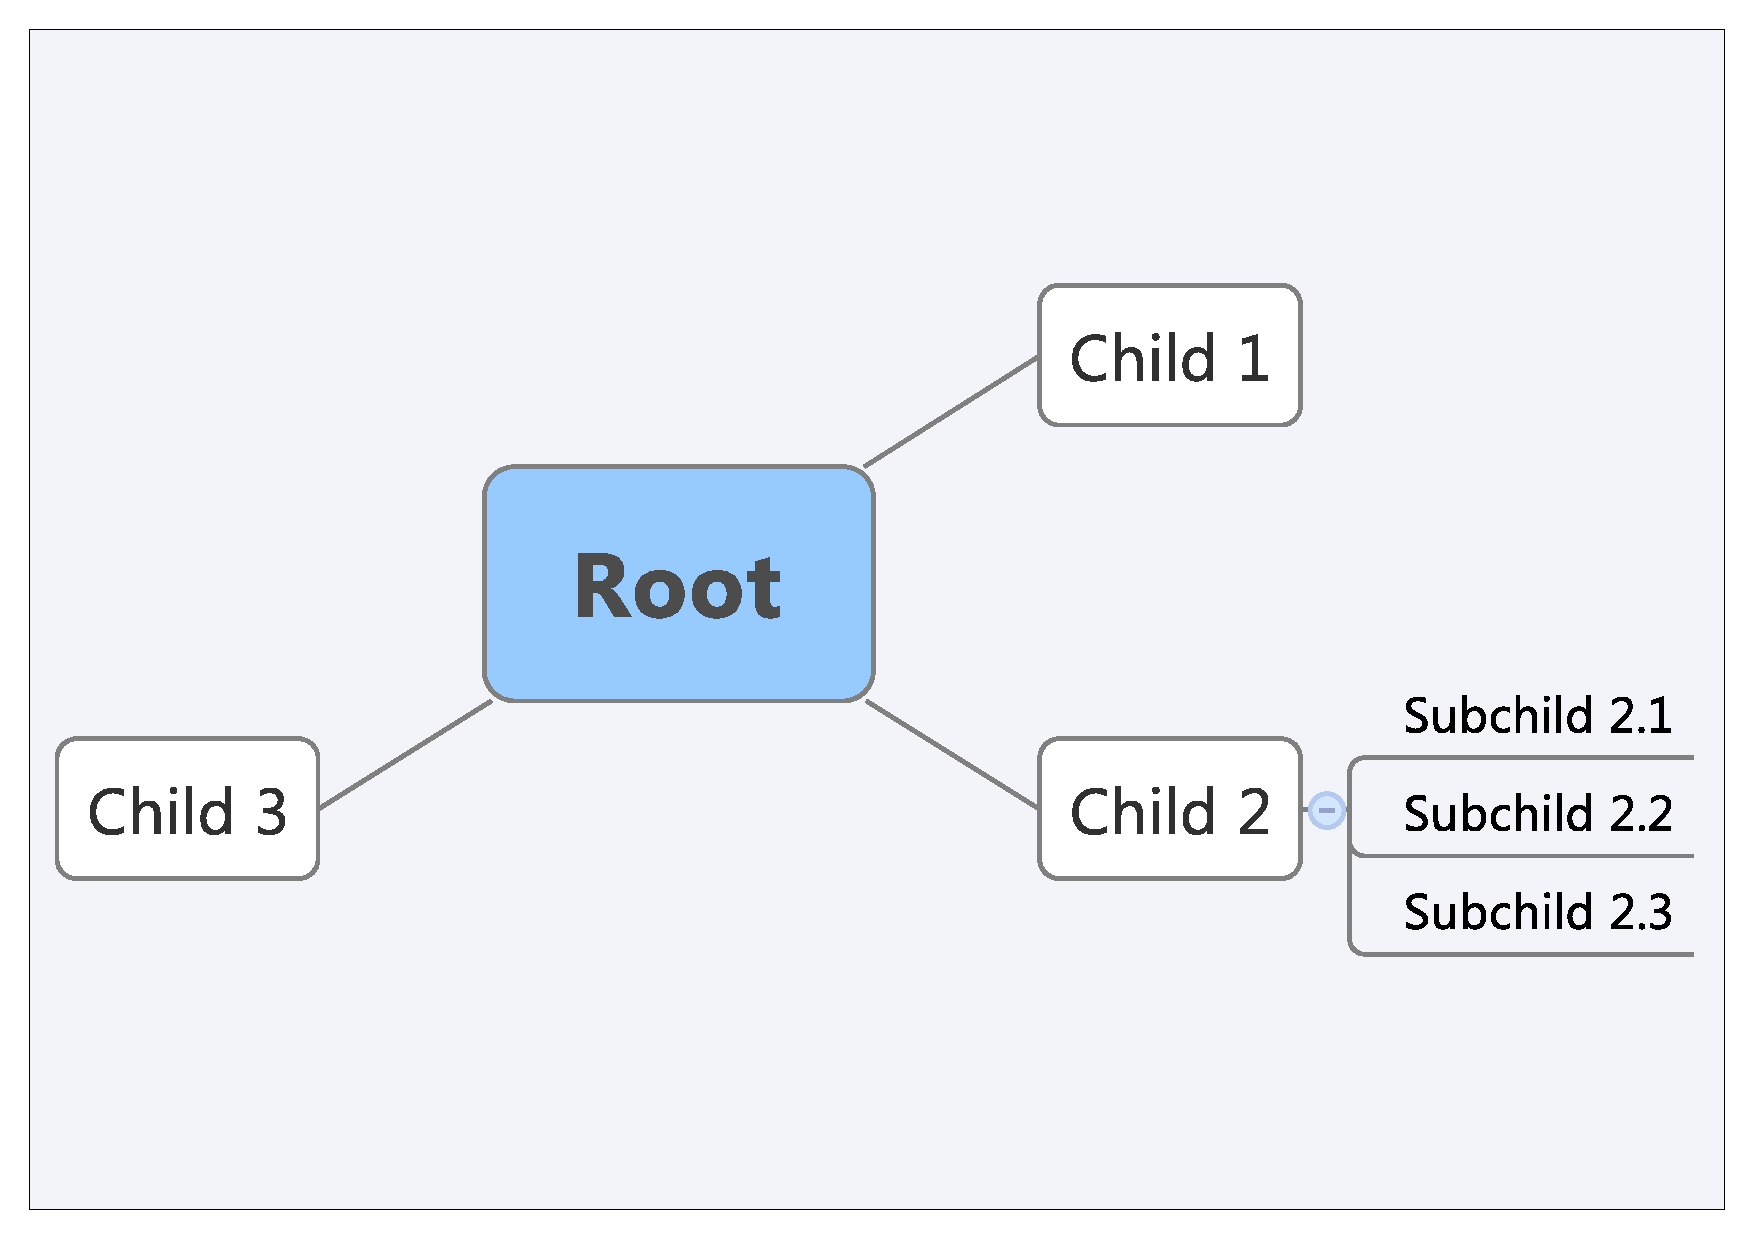
\includegraphics[width=\textwidth]{xmind}
			\caption{Mapa myśli z XMind-a.}
		\end{figure}
	\end{column}
\end{columns}



\end{frame}
